\documentclass[a4paper,11pt] {article}
\hfuzz=100pt 
%\documentclass[a4paper,article,oneside,10pt]{memoir}
\usepackage[latin1]{inputenc}
\usepackage[T1]{fontenc}
%\usepackage[lucidasmallscale, nofontinfo]{lucimatx}
%\usepackage{times}
\usepackage{graphicx}
\usepackage{longtable}
\usepackage{here}
\usepackage{ctable}
\usepackage{pdflscape}
\usepackage{pst-tree}
\usepackage{longtable}
\usepackage{multirow}
\usepackage{dcolumn}
\usepackage{Sweave}
\usepackage{lscape}
\usepackage{geometry}
\usepackage{graphicx}
\usepackage{subfig}
\usepackage{caption}
%\usepackage[pdftex,bookmarks=true,bookmarksnumbered=true,
%            hypertexnames=false,breaklinks=true,
%            linkbordercolor={0 0 1}]{hyperref}

%--------------

%
%\usepackage{fancyhdr}
%\pagestyle{empty}
%\pagestyle{fancy}
%\fancyhf{}
%%\renewcommand{\chaptermark}[1]{\markboth{\bsc{\chaptername~\thechapter{} :} #1}{}}
%%\renewcommand{\sectionmark}[1]{\markright{\thesection{} #1}}
%%\lfoot{Confidential, for the exclusive use of DMC members}
%%\renewcommand{\footrulewidth}{0.4pt}
%%\renewcommand{\headrulewidth}{0.4pt}
%%\renewcommand{\thepage}{\arabic{\page}}
%\setcounter{tocdepth}{5} % Dans la table des matieres
%\setcounter{secnumdepth}{5} % Avec un numero.
%%\mainmatter
%\pagenumbering{arabic}\setcounter{page}{1}
%\rhead{\thepage}
%\lhead{\leftmark}
%%\renewcommand{\thesection}{\Roman{section}}
%%\renewcommand{\thesection}{\Roman{section}}
%%\renewcommand{\thesection}{\Roman{section}}
%%\renewcommand{\thesubsection}{\thesection .\Alph{subsection}}
%
%--------------
\begin{document}
\title{Rapport  d'analyses statistiques}
\author{Axelle Dupont, sbim, Hopital Saint Louis, Paris}
\date{29 Mai 2017}

%------------------------------------------------------------






%-------------------------------------------------------------





\Sconcordance{concordance:Rapport.tex:Rapport.Rnw:%
1 109 1 1 50 4 1 1 9 69 0 1 2 1 9 16 0 1 2 1 1 1 9 129 0 1 2 2 1 1 9 58 %
0 1 2 8 1 2 12 1 11 7 1 2 2 10 1 2 2 10 1 1 4 8 1 2 2 11 1 2 2 5 1 1 4 %
14 1 1 4 7 1 1 4 8 1 1 4 4 1 1 4 12 1 1 5 5 1 1 6 7 1 1 11 8 1}



\setkeys{Gin}{width=1\textwidth}
\maketitle

%\pagestyle{protoc}
\tableofcontents
\pagebreak[4]
\listoftables
\listoffigures
%\SweaveOpts{eval=TRUE,echo=false,fig=TRUE}


\pagebreak[4]
%\chapter{Objectif}

\section{Objectives}

The primary objective of the study was to assess the survival, the risk of relapse and GVHD  of patients who underwent allogenic sterm-cell transplantation (alloSCT) for aggressive T-cell lymphomas. 
The second objective was to determine the variables associated with these outcomes.

\section{Methods}

A  retrospective analysis was conducted.A descriptive analysis of the variables recorded was perfomed. Different endpoints were defined : death, relapse, Event-free survival(EFS), Progression free Survival (PFC). Relapse was only considered in patients who had a complete remission after allo SCT.

Survival curves were estimated using Kaplan-Meier product-limit estimator.
Competing risk survival analysis methods were applied to estimate the cumulative incidence (CIF) of developing events over time from alloSCT. These methods allow for the fact that a patient may experience an event which is different from that of interest. These events are known as competing risk events, and may preclude the onset of the event of interest, or may modify the probability of the onset of that event.In particular, a transplanted patient may die before a relapse occurs. 

Factors associated with overall sur-vival were analyzed using Cox proportional hazards models. The proportional hazards assumption was checked by examination of Schoenfeld residuals.
For the different endpoints, univariable analyses were first carried out, then a multivariable analysis was used where all factors with P-value < 0.15 in the univariable analyses were considered. Factors where then sequentially removed from the adjusted model with a P-value cut- at 0.05. 
Survival is presented as estimate and 95\% confidence interval (95\% CI).


To test CIF between histopathologic groups we the test proposed by Gray. 

\pagebreak[4]
\section{Results}





\subsection{Descriptive results}
 285 patients were initially selected.We excluded 1 patient that underwent two alloSCT. The final analysis was perfomed on 284 patients and 284 grafts.
 \subsubsection{Patients characteristics}
% latex table generated in R 3.3.2 by xtable 1.8-2 package
% Mon May 29 13:09:49 2017
\begin{longtable}{llll}
  \hline
Parameters & Values & N & Statistics* \\ 
  \hline
 &  & 284 &  \\ 
  Age at diagnostic &  & 284 & 46.5 [36;55] \\ 
  Patient sex & Female & 93 & 32.75 \% \\ 
   & Male & 191 & 67.25 \% \\ 
  Age at diagnostic &  & 284 & 46.5 [36;55] \\ 
  Stage at diagnostic & I & 13 & 6.47 \% \\ 
   & II & 17 & 8.46 \% \\ 
   & III & 45 & 22.39 \% \\ 
   & IV & 126 & 62.69 \% \\ 
   & NA & 83 &  \\ 
  Stage at diagnostic & I-II & 113 & 39.79 \% \\ 
   & III-IV & 171 & 60.21 \% \\ 
  Subtypes & AITL & 82 & 28.87 \% \\ 
   & ALCL ALK- & 20 & 7.04 \% \\ 
   & ALCL ALK? & 2 & 0.7 \% \\ 
   & ALCL ALK+ & 21 & 7.39 \% \\ 
   & ATLL & 16 & 5.63 \% \\ 
   & EATL & 3 & 1.06 \% \\ 
   & HS & 12 & 4.23 \% \\ 
   & LGL & 1 & 0.35 \% \\ 
   & NK leukemia & 1 & 0.35 \% \\ 
   & NK/T nasal & 16 & 5.63 \% \\ 
   & NOS & 110 & 38.73 \% \\ 
  Subtypes & NOS & 110 & 38.73 \% \\ 
   & AITL & 82 & 28.87 \% \\ 
   & ALCL & 43 & 15.14 \% \\ 
   & ATLL & 16 & 5.63 \% \\ 
   & NK/T nasal & 16 & 5.63 \% \\ 
   & Others & 17 & 5.99 \% \\ 
  Centres & angers & 8 & 2.82 \% \\ 
   & Becquerel[941] & 4 & 1.41 \% \\ 
   & C.H.R.U Brest[659] & 2 & 0.7 \% \\ 
   & caen & 4 & 1.41 \% \\ 
   & CHU clermond ferrand & 7 & 2.46 \% \\ 
   & Geneve & 6 & 2.11 \% \\ 
   & Gustave Roussy[666] & 3 & 1.06 \% \\ 
   & H A Michallon[270] & 5 & 1.76 \% \\ 
   & H Bretonneau[272] & 3 & 1.06 \% \\ 
   & H Charles Nicolle[932] & 1 & 0.35 \% \\ 
   & H Claude Huriez[277] & 8 & 2.82 \% \\ 
   & H de l`ARCHET I[523]nice & 3 & 1.06 \% \\ 
   & H E Herriot[671] & 5 & 1.76 \% \\ 
   & H Haut-Leveque[267] & 31 & 10.92 \% \\ 
   & H Hautepierre[672] & 11 & 3.87 \% \\ 
   & H Jean Minjoz[233] & 5 & 1.76 \% \\ 
   & H La Miletrie[264] & 5 & 1.76 \% \\ 
   & H Mondor Hematol[252] & 4 & 1.41 \% \\ 
   & H Necker[160] & 9 & 3.17 \% \\ 
   & H Percy[665] & 4 & 1.41 \% \\ 
   & H Purpan[624] & 8 & 2.82 \% \\ 
   & H Sud/Pontchaillou[661] & 7 & 2.46 \% \\ 
   & H Sud[955] & 1 & 0.35 \% \\ 
   & Hotel Dieu[253] & 32 & 11.27 \% \\ 
   & liege & 8 & 2.82 \% \\ 
   & limoges & 3 & 1.06 \% \\ 
   & montpellier & 10 & 3.52 \% \\ 
   & nancy & 1 & 0.35 \% \\ 
   & Paoli Calmettes[230] & 39 & 13.73 \% \\ 
   & Pellegrin-Enfants[978] & 1 & 0.35 \% \\ 
   & Pitie-Salpetrriere[262] & 8 & 2.82 \% \\ 
   & St Antoine[775] & 10 & 3.52 \% \\ 
   & St Etienne[250] & 4 & 1.41 \% \\ 
   & St Louis[207] & 24 & 8.45 \% \\ 
   \hline
\hline
\caption{Patients characteristics} 
\label{tab:condi}
\end{longtable} \subsubsection{Treatments before alloSCT}
% latex table generated in R 3.3.2 by xtable 1.8-2 package
% Mon May 29 13:09:49 2017
\begin{longtable}{llll}
  \hline
Parameters & Values & N & Statistics* \\ 
  \hline
 &  & 284 &  \\ 
  Previous auto & No & 191 & 67.25 \% \\ 
   & Yes & 93 & 32.75 \% \\ 
   Programme auto allo & No & 257 & 90.49 \% \\ 
   & Yes & 27 & 9.51 \% \\ 
  First graft relapse & No & 219 & 77.11 \% \\ 
   & Yes & 65 & 22.89 \% \\ 
   \hline
\hline
\caption{Treatments before alloSCT} 
\label{tab:avtg}
\end{longtable}\pagebreak
 \subsubsection{Transplant conditions}
% latex table generated in R 3.3.2 by xtable 1.8-2 package
% Mon May 29 13:09:49 2017
\begin{longtable}{llll}
  \hline
Parameters & Values & N & Statistics* \\ 
  \hline
 &  & 284 &  \\ 
  Age at graft &  & 284 & 49.5 [38;57] \\ 
  Age at graft & < 49 years & 139 & 48.94 \% \\ 
   & > 49 years & 145 & 51.06 \% \\ 
  Donor age &  & 263 & 28 [18;39] \\ 
  Donor sex & Female & 114 & 40.71 \% \\ 
   & Male & 166 & 59.29 \% \\ 
   & NA & 4 &  \\ 
  Delay diagnosis and allo SCT &  & 284 & 378.5 [213.2;710.8] \\ 
  >12 months delay & NO & 149 & 52.46 \% \\ 
   & Yes & 135 & 47.54 \% \\ 
  Stage at diagnostic & I & 13 & 6.47 \% \\ 
   & II & 17 & 8.46 \% \\ 
   & III & 45 & 22.39 \% \\ 
   & IV & 126 & 62.69 \% \\ 
   & NA & 83 &  \\ 
  Disease status at transplant & CR/PR & 251 & 88.69 \% \\ 
   & PD & 32 & 11.31 \% \\ 
   & NA & 1 &  \\ 
  Disease status at transplant & CR & 175 & 61.84 \% \\ 
   & PD & 32 & 11.31 \% \\ 
   & PR & 76 & 26.86 \% \\ 
   & NA & 1 &  \\ 
  Disease status at transplant & CR (?) & 7 & 2.47 \% \\ 
   & CR1 & 94 & 33.22 \% \\ 
   & CR2 & 61 & 21.55 \% \\ 
   & CR3 & 13 & 4.59 \% \\ 
   & PD & 32 & 11.31 \% \\ 
   & PR (?) & 13 & 4.59 \% \\ 
   & PR1 & 39 & 13.78 \% \\ 
   & PR2 & 18 & 6.36 \% \\ 
   & PR3 & 5 & 1.77 \% \\ 
   & PR4 & 1 & 0.35 \% \\ 
   & NA & 1 &  \\ 
  Karnofsky &  & 263 & 90 [80;100] \\ 
  Karnofsky & 100 & 92 & 34.98 \% \\ 
   & 40 & 1 & 0.38 \% \\ 
   & 50 & 4 & 1.52 \% \\ 
   & 60 & 1 & 0.38 \% \\ 
   & 70 & 9 & 3.42 \% \\ 
   & 80 & 70 & 26.62 \% \\ 
   & 90 & 86 & 32.7 \% \\ 
   & NA & 21 &  \\ 
  No of lines before alloSCT &  & 284 & 30 [165;NA] \\ 
  No of lines before alloSCT & 1 & 73 & 28.74 \% \\ 
   & 2 & 92 & 36.22 \% \\ 
   & 3 & 65 & 25.59 \% \\ 
   & >=4 & 24 & 9.45 \% \\ 
   & NA & 30 &  \\ 
  Donnor related & Yes & 149 & 52.46 \% \\ 
   & No & 135 & 47.54 \% \\ 
  HLA match & Yes & 53 & 18.66 \% \\ 
   & No & 231 & 81.34 \% \\ 
  HLA match & Identical sibling & 128 & 45.07 \% \\ 
   & Matched unrelated & 103 & 36.27 \% \\ 
   & Mismatched relative & 7 & 2.46 \% \\ 
   & Mismatched unrelated & 13 & 4.58 \% \\ 
   & Unrelated CB & 33 & 11.62 \% \\ 
  sex of patient/donnor & M/F & 47 & 16.55 \% \\ 
   & Others & 237 & 83.45 \% \\ 
  CMV serostatus of patient/donnor & neg/pos & 52 & 18.31 \% \\ 
   & Others & 232 & 81.69 \% \\ 
  Source of stem cells & BM & 49 & 17.25 \% \\ 
   & CB & 33 & 11.62 \% \\ 
   & PB & 202 & 71.13 \% \\ 
  TBI & No & 161 & 56.69 \% \\ 
   & Yes & 123 & 43.31 \% \\ 
  conditioning Intensity & MAC & 106 & 38.13 \% \\ 
   & NMA & 27 & 9.71 \% \\ 
   & RIC & 145 & 52.16 \% \\ 
   & NA & 6 &  \\ 
  Conditioning & BEAM & 1 & 0.36 \% \\ 
   & BEAM + Campath & 1 & 0.36 \% \\ 
   & BU CY  & 4 & 1.42 \% \\ 
   & BU CY + FLU+ ATG & 1 & 0.36 \% \\ 
   & BU CY ATG & 1 & 0.36 \% \\ 
   & EDX ATG & 0 & 0 \% \\ 
   & ENX TBI 2gray & 1 & 0.36 \% \\ 
   & FLU ATG & 3 & 1.07 \% \\ 
   & FLU BU 1+ ATG & 3 & 1.07 \% \\ 
   & FLU BU 2 & 1 & 0.36 \% \\ 
   & FLU BU 2+ ATG & 73 & 25.98 \% \\ 
   & FLU BU 3+ ATG & 21 & 7.47 \% \\ 
   & FLU BU 4+ ATG & 10 & 3.56 \% \\ 
   & FLU BU EDX & 8 & 2.85 \% \\ 
   & FLU BU EDX +ATG & 6 & 2.14 \% \\ 
   & FLU EDX & 1 & 0.36 \% \\ 
   & FLU EDX ATG & 3 & 1.07 \% \\ 
   & FLU EDX MEL & 1 & 0.36 \% \\ 
   & FLU ENX TBI 2gray & 24 & 8.54 \% \\ 
   & FLU ENX TBI 4gray & 2 & 0.71 \% \\ 
   & FLU ENX TBI 6gray & 1 & 0.36 \% \\ 
   & FLU ENX TBI 6gray + campath & 1 & 0.36 \% \\ 
   & FLU MEL & 12 & 4.27 \% \\ 
   & FLU MEL + campath & 4 & 1.42 \% \\ 
   & FLU MEL + Campath & 1 & 0.36 \% \\ 
   & FLU MEL ATG & 1 & 0.36 \% \\ 
   & FLU MEL TBI 2gray & 1 & 0.36 \% \\ 
   & FLU TBI 2gray & 21 & 7.47 \% \\ 
   & FLU TBI 2gray ATG & 1 & 0.36 \% \\ 
   & FLU Tbi 8 gray & 1 & 0.36 \% \\ 
   & MEL 140 TBI 10 gray & 1 & 0.36 \% \\ 
   & MEL TBI VP16 & 1 & 0.36 \% \\ 
   & TB2F & 2 & 0.71 \% \\ 
   & TBI 12 gray & 1 & 0.36 \% \\ 
   & TBI 2gray & 1 & 0.36 \% \\ 
   & TBI EDX & 49 & 17.44 \% \\ 
   & TBI EDX +ATG & 11 & 3.91 \% \\ 
   & TBI EDX FLU & 5 & 1.78 \% \\ 
   & Thiotepa etoposide TBI12 gray & 1 & 0.36 \% \\ 
   & NA & 3 &  \\ 
  Cells manipulation & No & 275 & 97.86 \% \\ 
   & Yes & 6 & 2.14 \% \\ 
   & NA & 3 &  \\ 
  No of donnors & 1 & 261 & 91.9 \% \\ 
   & 2 & 23 & 8.1 \% \\ 
   \hline
\hline
\caption{Transplant conditions} 
\label{tab:g}
\end{longtable}
\pagebreak
\subsubsection{Post-AlloSCT Response}
% latex table generated in R 3.3.2 by xtable 1.8-2 package
% Mon May 29 13:09:50 2017
\begin{longtable}{llll}
  \hline
Parameters & Values & N & Statistics* \\ 
  \hline
 &  & 284 &  \\ 
  Agvhd & No & 141 & 49.65 \% \\ 
   & Yes & 143 & 50.35 \% \\ 
  Agvhd grade & No aGvHD present (Grade 0) & 141 & 49.65 \% \\ 
   & Grade I & 49 & 17.25 \% \\ 
   & Grade II & 46 & 16.2 \% \\ 
   & Grade III & 24 & 8.45 \% \\ 
   & Grade IV & 17 & 5.99 \% \\ 
   & Present, grade unknown & 7 & 2.46 \% \\ 
  Cgvhd & No & 187 & 65.85 \% \\ 
   & Yes & 97 & 34.15 \% \\ 
  Cgvhd grade & Early death (100D) & 41 & 14.44 \% \\ 
   & Extensive & 38 & 13.38 \% \\ 
   & Limited & 55 & 19.37 \% \\ 
   & No cGvh & 146 & 51.41 \% \\ 
   & grade unknown & 4 & 1.41 \% \\ 
  Engrafted & Early death (30D) & 5 & 1.76 \% \\ 
   & Engrafted & 271 & 95.42 \% \\ 
   & Lost graft & 2 & 0.7 \% \\ 
   & No engraftment & 6 & 2.11 \% \\ 
  Cause of death & HSCT-GVHd & 21 & 19.63 \% \\ 
   & HSCT-GVHd + infection & 3 & 2.8 \% \\ 
   & HSCT-infection & 27 & 25.23 \% \\ 
   & HSCT-toxicity & 4 & 3.74 \% \\ 
   & HSCT related & 3 & 2.8 \% \\ 
   & HSCT related ILD & 1 & 0.93 \% \\ 
   & HSCT related MAT & 1 & 0.93 \% \\ 
   & HSCT related MOF & 2 & 1.87 \% \\ 
   & HSCT related MVO & 1 & 0.93 \% \\ 
   & HSCT related pneumopathie interstititelle & 2 & 1.87 \% \\ 
   & HSCT related PTLD & 1 & 0.93 \% \\ 
   & HSCT related SDRA & 1 & 0.93 \% \\ 
   & Other & 1 & 0.93 \% \\ 
   & Relapse or progression of original disease & 37 & 34.58 \% \\ 
   & Secondary malignancy & 1 & 0.93 \% \\ 
   & Unknown & 1 & 0.93 \% \\ 
   & NA & 177 &  \\ 
  Best reponse after SCT & CR & 245 & 86.88 \% \\ 
   & Not evaluable & 4 & 1.42 \% \\ 
   & Not evaluated & 3 & 1.06 \% \\ 
   & PD & 14 & 4.96 \% \\ 
   & PR & 16 & 5.67 \% \\ 
   & NA & 2 &  \\ 
  Relapse/progression & Continuous progression & 28 & 9.93 \% \\ 
   & No & 217 & 76.95 \% \\ 
   & Non applicable  & 3 & 1.06 \% \\ 
   & Yes & 34 & 12.06 \% \\ 
   & NA & 2 &  \\ 
  Death & Alive & 177 & 62.32 \% \\ 
   & Dead & 107 & 37.68 \% \\ 
   \hline
\hline
\caption{Post-AlloSCT Response} 
\label{tab:pg}
\end{longtable}


\pagebreak[4]
\newgeometry{bmargin=1cm}
\begin{landscape}





\end{landscape}

\restoregeometry

\subsection{Survival analysis}
Median follow-up from the date of AlloSCT was 20.35 (range 0.03 to 113.77). OS at 1 year was 0.68 (95 \% 0.63 - 0.74), was 0.64 (95 \% 0.59 - 0.7) at 2 years
.OS at 4 years was 0.57 (95 \% 0.5 - 0.64).
\begin{figure}[h]
\begin{center}
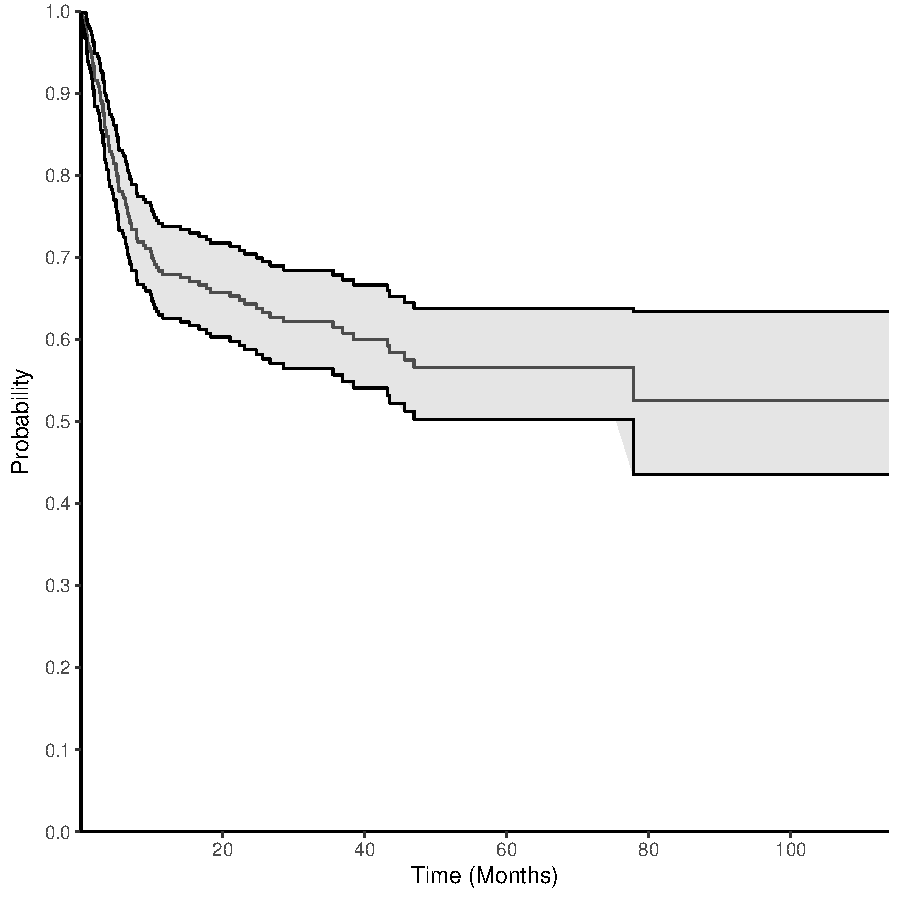
\includegraphics{Rapport-fig1}
\end{center}
\caption{Overall survival}
\label{fig1}
\end{figure}

\pagebreak
EFS at 1 year was 0.54 (95 \% 0.48 - 0.6), was 0.49 (95 \% 0.43 - 0.55) at 2 years. EFS at 4 years was 0.42 (95 \% 0.36 - 0.5).

\begin{figure}[h]
\begin{center}
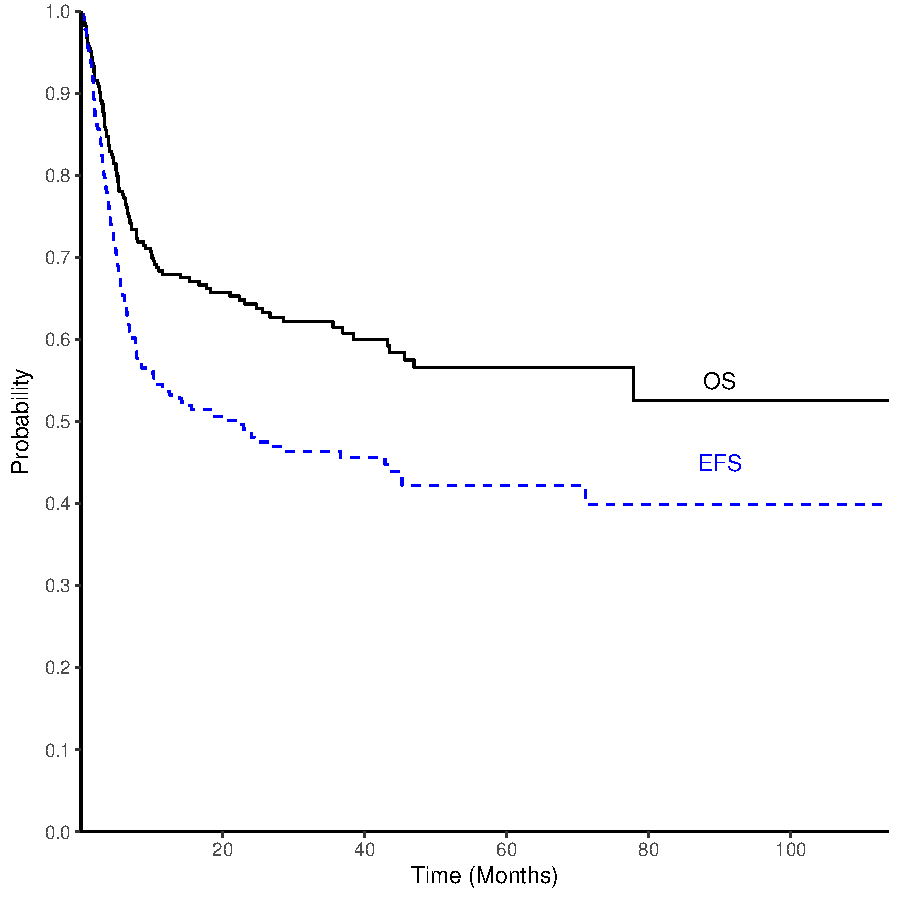
\includegraphics{Rapport-fig2}
\end{center}
\caption{Event-free survival}
\label{fig2}
\end{figure}

\pagebreak
PFS at 1 year was 0.73 (95 \% 0.65 - 0.83), was 0.68 (95 \% 0.59 - 0.78) at 2 years. PFS at 4 years was 0.66 (95 \% 0.56 - 0.77).

\begin{figure}[h]
\begin{center}
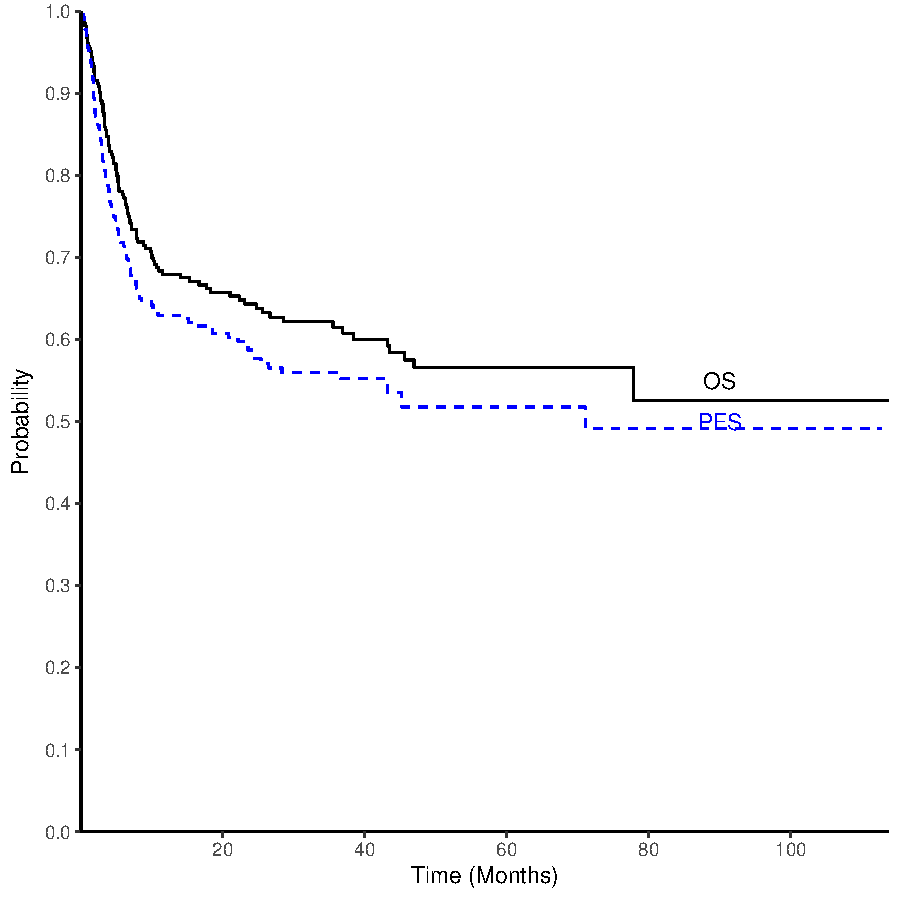
\includegraphics{Rapport-fig3}
\end{center}
\caption{Progression-free survival}
\label{fig3}
\end{figure}

\pagebreak
Relapse at 1 year was 0.87 (95 \% 0.83 - 0.92), was 0.85 (95 \% 0.8 - 0.9) at 2 years. Relapse at 4 years was 0.83 (95 \% 0.77 - 0.89).
\\
\begin{center}
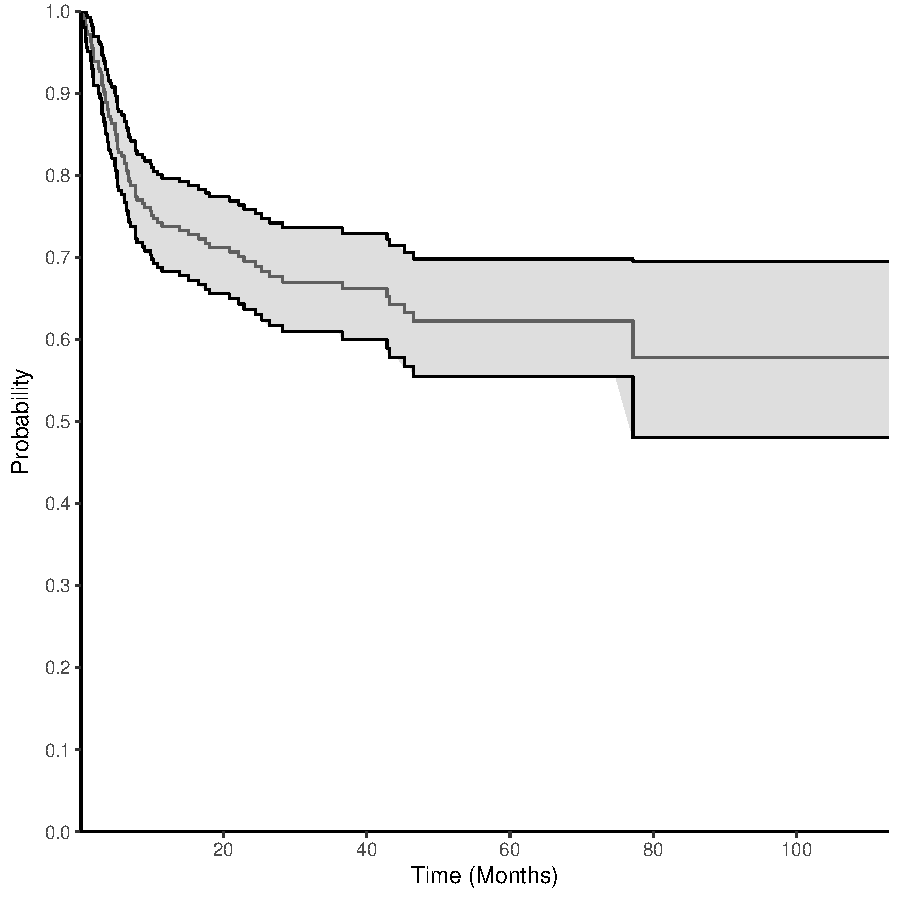
\includegraphics[width=0.5\textwidth]{C:/Users/adupont/Documents/projetstlouis/scripts/Rapport-figg.pdf}
\captionof{figure}{Relapse in patients with a complete remission post alloSCT}

\end{center}
\begin{center}
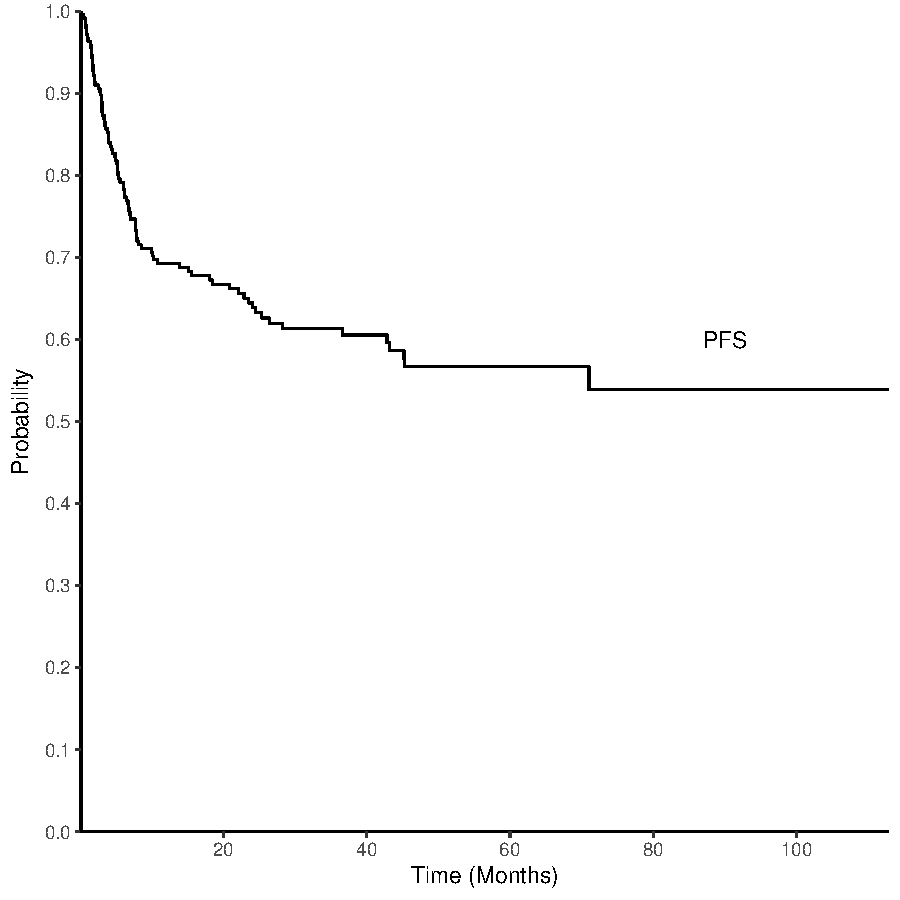
\includegraphics[width=0.5\textwidth]{C:/Users/adupont/Documents/projetstlouis/scripts/Rapport-figg2.pdf}
\captionof{figure}{PFS in patients with a complete remission post alloSCT}

\end{center}
\begin{center} 
 
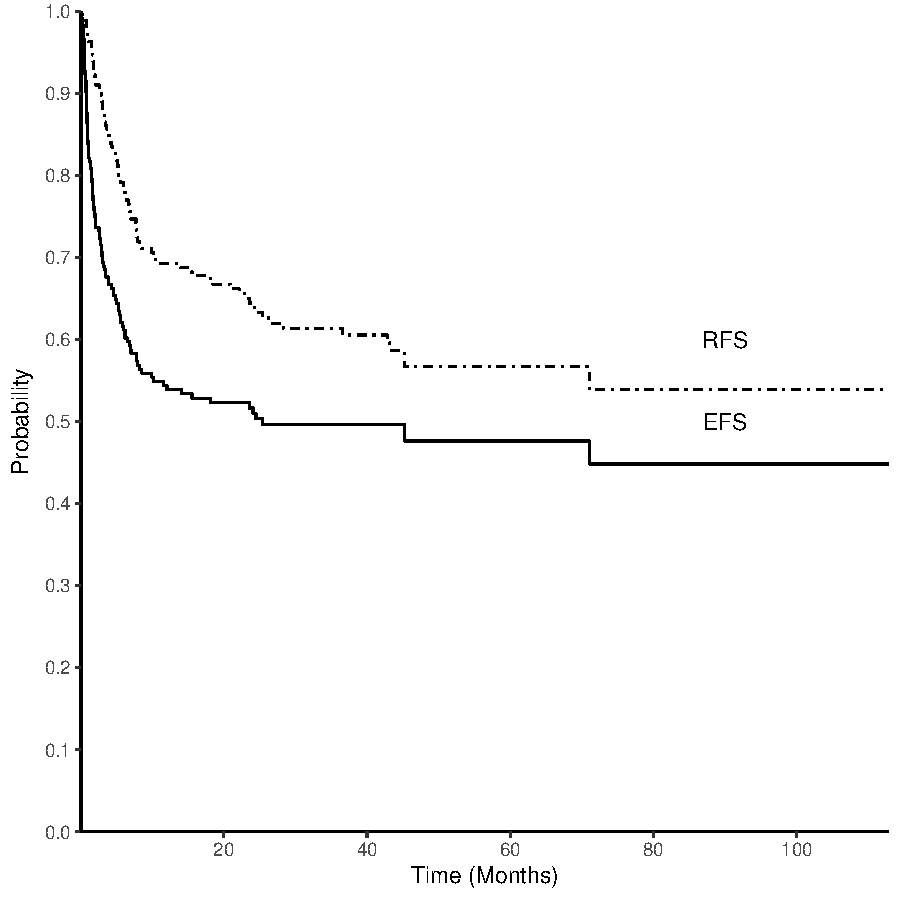
\includegraphics[width=0.5\textwidth]{C:/Users/adupont/Documents/projetstlouis/scripts/Rapport-xcube.pdf}
\captionof{figure}{EFS in patients with a complete remission post alloSCT}



\end{center}
\pagebreak
CIF for related HSCT death at 1 years was 0.2, at 2 years  0.22.
CIF for non-related HSCT Death at 1 year was 0.12, at 2 years  0.13.
\begin{figure}[h]
\begin{center}
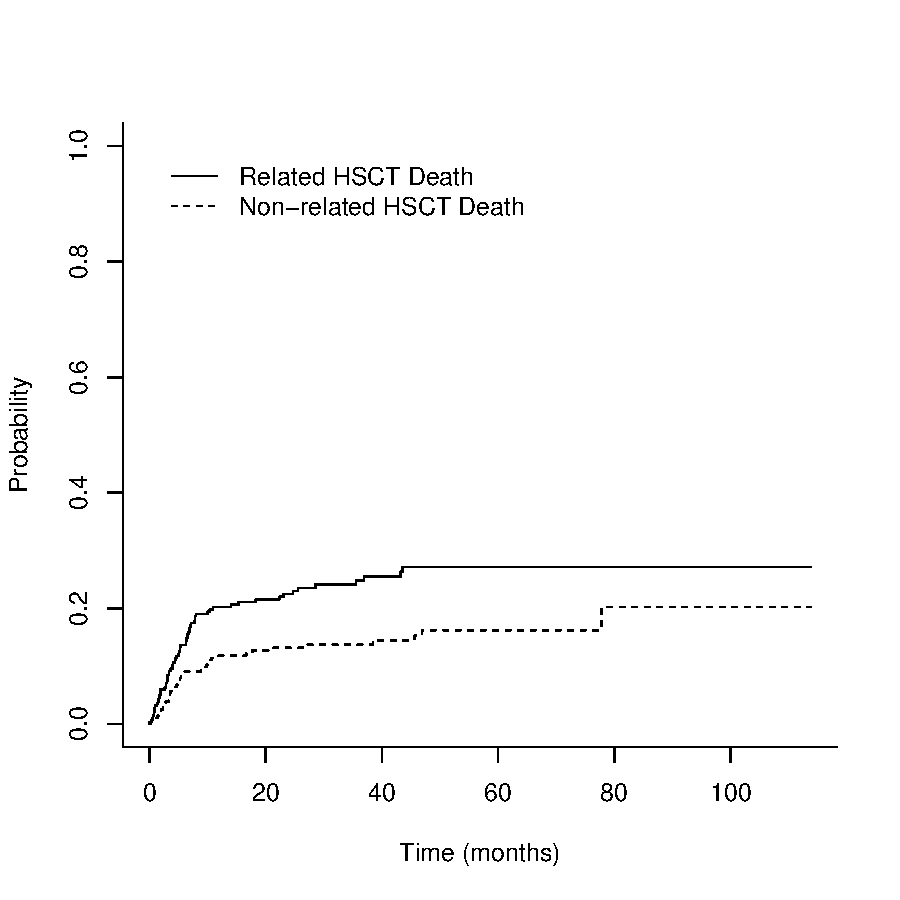
\includegraphics{Rapport-fig5}
\end{center}
\caption{CIF of Related HSCT Death and Non-related HSCT Death}
\label{fig5}
\end{figure}

\pagebreak
CIF for relapse/progression at 1 years was 0.18, at 2 years  0.19.
CIF for death without relapse or progression at 1 year was 0.19, at 2 years  0.22. 

\begin{figure}[h]
\begin{center}
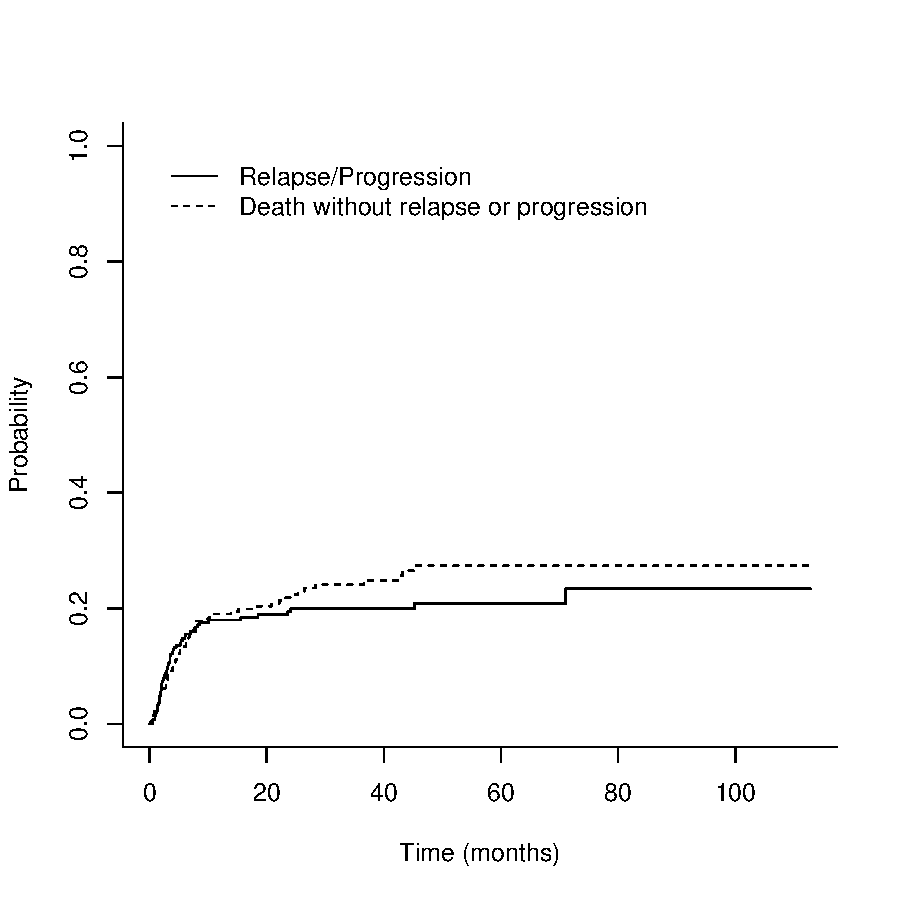
\includegraphics{Rapport-fig6}
\end{center}
\caption{CIF of relapse or progression and death without relapse or progression}
\label{fig6}
\end{figure}

\pagebreak
CIF for relapse at 1 year was 0.12, at 2 years  0.13. CIF for death without relapse  at 1 year was 0.19, at 2 years  0.22. 


\begin{center}
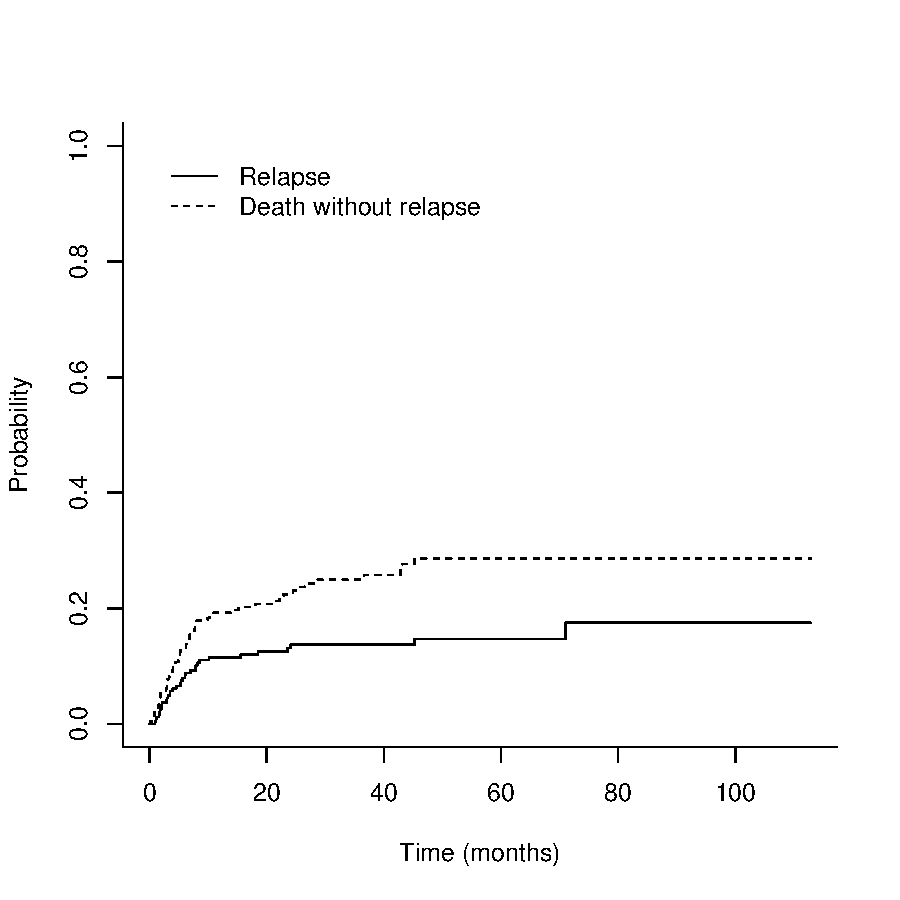
\includegraphics[width=0.8\textwidth]{C:/Users/adupont/Documents/projetstlouis/scripts/Rapport-fig7.pdf}
\captionof{figure}{CIF of relapse and death without relapse (in patients with a complete remission post alloSCT)}


\end{center}

\subsection{Univariate Analysis}




% latex table generated in R 3.3.2 by xtable 1.8-2 package
% Fri May 26 14:16:17 2017




\end{document}
